\documentclass[conference]{IEEEtran}
\IEEEoverridecommandlockouts

\usepackage{cite}
\usepackage{tabularray}
\usepackage{amsmath,amssymb,amsfonts}
\usepackage{tikz}
\usetikzlibrary{arrows.meta, positioning}
\usepackage{hyperref}
\usepackage{graphicx}
\usepackage{textcomp}
\usepackage{xcolor}
\usepackage{algorithm}
% \usepackage{algorithmic}
\usepackage{algpseudocode}
\usepackage{caption}
\usepackage{xurl}
\usepackage{pgfplots}
\pgfplotsset{tick label style={/pgf/number format/fixed}}

\pgfplotsset{compat=1.18}

\def\BibTeX{{\rm B\kern-.05em{\sc i\kern-.025em b}\kern-.08em
    T\kern-.1667em\lower.7ex\hbox{E}\kern-.125emX}}
\begin{document}

\title{ Kernel-Level Semantic Search with Knowledge Graphs
}

\author{\IEEEauthorblockN{}
\and
\IEEEauthorblockN{Arjun Deodhar}
\IEEEauthorblockA{\textit{Department of CSE} \\
\textit{COEP Technological University} \\
Pune, Maharashtra, India \\
arjundeodhar@gmail.com\\
deodhark22.comp@coeptech.ac.in} 
\and
\IEEEauthorblockN{Arnav Prasad}
\IEEEauthorblockA{\textit{Department of CSE} \\
\textit{COEP Technological University} \\
Pune, Maharashtra, India \\
arnav.prasad.ap@gmail.com\\
arnavp22.comp@coeptech.ac.in}
\and
\IEEEauthorblockN{Prajwal Bhosale}
\IEEEauthorblockA{\textit{Department of CSE} \\
\textit{COEP Technological University} \\
Pune, Maharashtra, India \\
pjlbhosale@gmail.com\\
bhosalepp22.comp@coeptech.ac.in}
}

\maketitle

\begin{abstract}
Various types of knowledge exist across individuals, processes, and tools.
The chief objective of Knowledge Graph (KG) is to aggregate the data into graph format, ensuring that it remains manageable, non-corrupted, scalable, and easily discoverable.

At its core, a KG is a structure where each node represents real-world entities and edges logically depict the relationships between the nodes. The graph can be directed or un-directed, depending on the organization's needs. Our approach involves a directed graph that also includes backward edges!

The end objective of KG is to operationalize Knowledge (a piece of information) at the kernel level and make it available to users when they feed specific queries to the graph. The output should be the most relevant and concise response available, neither too lengthy nor too brief.
\end{abstract}

\begin{IEEEkeywords}
\textit{Knowledge Graph, kernel-level implementation, AVL, heap}
\end{IEEEkeywords}

\subsection{Abbreviations and Acronyms}\label{AA}

\begin{itemize}
    \item \textbf{KGs}: Knowledge Graphs
    \item \textbf{AVL}: Adelson-Velsky and Landis
    \item \textbf{max\_heap}: maximum heap
    \item \textbf{NLP}: Natural Language Processing
    \item \textbf{CSV}: Comma Separated Value
\end{itemize}


\section{INTRODUCTION}
KGs are advanced data structures. They are designed to facilitate and improve information retrieval, question-answering, and semantic search capabilities.
The concept of the KG gained significant recognition in 2012 when Google \cite{b7} publicly credited their search solution to the use of KG.


\begin{figure}[htbp]
\centering
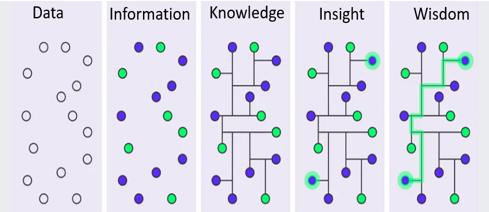
\includegraphics[width=0.8\linewidth , height=3cm]{intro_dots_image_kg.png }
\caption{Transforming Raw Data\cite{b1} into Knowledge}
\label{fig}
\end{figure}


The relationships in KG are often labeled to provide context and meaning, forming a rich, structured representation of knowledge.
They support direct and inferred relationships, enabling more sophisticated reasoning and inference.
\\KGs have various applications : 
\begin{itemize}
    \item \textbf{E-Commerce}: Widely used by platforms like Amazon\cite{b2, b3} and eBay\cite{b4} to describe and categorize products for sale.
    \item \textbf{Social Networking}: Utilized by platforms such as LinkedIn\cite{b5} to manage and connect users, jobs, skills, and more.
\end{itemize}


The primary contributions of this study are summarized as follows:

\begin{itemize}
    \item It introduces a structural framework for constructing a KG at the kernel level without relying on external libraries.
    \item The developed KG can manage diverse types of queries, providing precise and relevant responses.
    % \item The algorithm presented in this paper has been tested and analyzed on a large fabricated dataset of inputs, demonstrating robust and effective performance.
    \item The algorithm presented in this paper has been evaluated and analyzed using a substantial fabricated dataset of inputs. For querying on a KG (dataset size: 917,568 lines of data), each query operation takes 0.174399 seconds.
\end{itemize}

After reviewing various research papers, many of them included the abstract concept of KG, but they lacked detailed structural implementation at the kernel level. 
Consequently, there arose a need to construct a fabricated input data set \cite{b11}, which is provided in the GitHub link.\\
The paper aims to provide a road-map for a thorough exploration of the fundamental implementation aspects of KGs.


The paper is structured as follows:

% \begin{itemize}
%     \item \textbf{Section 2}: Introduces the relevant work and study on KG in the literature.
%     \item \textbf{Section 3}: Describes the real-world data that should be handled by KG.
%     \item \textbf{Section 4}: Explains the proposed memory architecture of KG and its data structures.
%     \item \textbf{Section 5}: Demonstrates the proposed data flow in KG.
%     \item \textbf{Section 6}: Elaborates on analyzing the algorithms used in KG.
%     \item \textbf{Section 7}: Presents the pseudo-code of the algorithms.
%     \item \textbf{Section 8}: Includes the results and performance analysis of KG.
%     \item \textbf{Section 9}: Concludes the study.
% \end{itemize}


Section 2 Introduces the relevant work and study on KG in the literature. Section 3 Describes the real-world data that should be handled by KG. Section 4 Explains the proposed memory architecture of KG and its data structures. Section 5 Demonstrates the proposed data flow in KG. Section 6 Elaborates on analyzing the algorithms used in KG. Section 7 Presents the pseudo-code of the algorithms. Section 8 Includes the results and performance analysis of KG.
Finally, Section 9 Concludes the study.


\section{LITERATURE SURVEY}

Aidan Hogan et al\cite{b8} suggested concepts of KG such as graph modeling, ontologies, deductive knowledge, graph embeddings, and more. The paper features a rich bibliography with over 400 references.
With reference to \cite{b8}, we studied various graph models, including heterogeneous graphs\cite{b18}, property graphs\cite{b12}, and directed-edge labeled graphs\cite{b8}. This paper delves into the implementation of directed-edge labeled weighted graphs with further additions and improvements.
\\
Ergeta Muca\cite{b7} outlined the types of data sources commonly used for KG as structured inputs. The paper emphasized the advantages of KGs over traditional databases.It explained the concept of KGs, their origin, and highlighted their key applications.

Samadrita Ghosh \cite{b1} puts forward the concept of KGs, highlighting the key differences between a "graph" and a "Knowledge Graph." It also discusses the relationship between KGs and artificial intelligence.

Helena Cousijn, Ricarda Braukmann, et al. \cite{b16} presented and highlighted the concept and importance of "identity" in the context of data parsing and extraction.

Liu, Yu, and Hua \cite{b17} summarized the concept of temporal context.

These insights from the literature review inspired the authors to present the structural implementation and significance of KGs.



\section{METHODOLOGY}
Data can be of variable length, context, grammar, etc.
\\A KG is not just a collection of data  \cite{b8} but also contains hierarchical structures, contexts for data, as well as unique identifiers for real word entities.
\\
The constructed KG should be able to handle and recognize the following characteristics of data:
\begin{itemize}
    \item\textbf{Context of entities.}\cite{b8}\\ 
    For example, if the word "bank" is considered, the context can be a river-side bank or bank that involves financial transactions, or specifically Bank of Maharashtra, or may have some other context.
    

    
	\item\textbf{Weight of the connection}
 \\
 The connection with the highest weight should be displayed first.
The text analyzer should be able to assign front and back weights accordingly. For example, consider the sentence: "Arjun plays piano". This may be an important attribute for "Arjun" but not that relevant for "piano" (i.e. piano is being played by "Arjun" and piano will have more important (weighted) characteristics). 

 
	\item\textbf{Temporal constraints} \cite{b8, b17}
 \\
 For example, the statement "XYZ is the Prime Minister of India" will be valid only for a certain period (say five years) and after that, it may change. After expiration, the relation should be redundant.

 
	\item\textbf{Identity} \cite{b8,b16}
 \\
 For example, "Arjun plays piano" and "Arjun plays guitar", although the name "Arjun" has been repeated, in the real world, it may refer to different entities. 
 The analyzer should assign unique identifiers to different entities.
	
 \item\textbf{Misspelled Words Queries} 
 \\
 The query analyzer should be able to detect spelling errors in input queries and deliver the correct output by prompting the matching entities.
 
\end{itemize}

To accomplish all these features, the designed input data set contains the following fields: front-weight, inference, truth-bit, noun1, noun1\_id, verb, verb descriptor, noun2, noun2\_id, back-weight, definition, end-time.


\section{PROPOSED ARCHITECTURE}

\subsection{\textbf{Data Structures Used}}
The implementation in C programming language\cite{b9}, employs structures and pointers for AVL trees and arrays for heaps, providing a robust framework for managing non-centric knowledge representations and their interconnections via verbs.

\subsubsection{\textbf{AVL Tree}}

AVL trees are among the most efficient data structures for searching and inserting nodes(data) due to their 
self-balancing nature. The predictable performance of AVL trees makes them a powerful and widely used choice in computer science.
The insertion and search operations in an AVL tree have a time complexity of $O(\lg n)$, 
where "n" represents the number of nodes that are already present in the AVL tree.


\subsubsection{\textbf{Maximum Heap}}

Max\_heaps are highly efficient data structures for managing and retrieving the maximum weighted element. 
The most weighted element is always at the root enabling $O(1)$ time complexity for retrieval

Inserting and deleting elements in a max heap has $O(\lg n)$ time complexity.

All these make max\_heap quite useful in applications like scheduling algorithms, resource management, and real-time simulations.


\subsection{\textbf{Structural Implementation}}

\subsubsection{\textbf{Central Noun Tree}}
The core of our KG is an AVL tree where each node represents a noun. Each noun node comprises the following elements:
\begin{itemize}

    \item \textit{noun\_name}: Pointer to a string representing the noun.
    \item \textit{noun\_id}: A unique identifier for the noun.
    \item \textit{noun\_definition}: Pointer to a string containing the definition of the noun.
    \item \textit{next\_verb\_tree}: An AVL tree containing verbs that form front links to other nouns.
    \item \textit{prev\_verb\_tree}: Pointer to an AVL tree containing verbs that form back-links to other nouns.
    \item \textit{search\_max\_heap}: A max\_heap for extracting the highest priority connections.
    \item \textit{subclass\_max\_heap}: A max\_heap for accessing the highest priority sub-classes of the noun.
    \item \textit{left, right, balance\_factor}: for maintaining AVL tree. 
    
\end{itemize}

% \begin{figure}[htbp]
% \centering
% 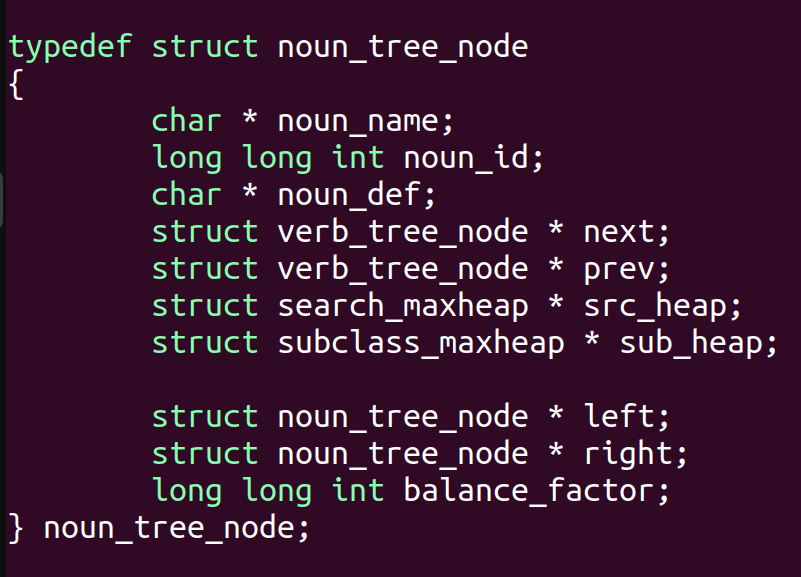
\includegraphics[width=0.8\linewidth , height=5cm]{vi_editor_typedef.png}
% \caption{Structural implementation in C}
% \label{fig}
% \end{figure}


% \begin{figure}[htbp]
% \centering
% 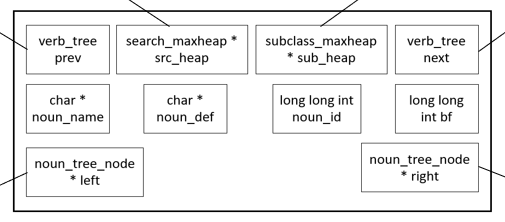
\includegraphics[width=0.8\linewidth]{noun_tree_node_pointer_diagram.png} % Adjust the width as needed
% \caption{Figure shows Structure diagram for Central Noun Tree node.}
% \label{fig}
% \end{figure}

\subsubsection{\textbf{Prev and Next Verb Trees}}
As explained, each noun\_tree node has its own next and previous verb\_trees. These contain connections to edges as well as some information about the verb being stored. Each verb\_tree node comprises of:

\begin{itemize}

    \item \textit{verb\_name}: Pointer to a string in the database tree of verbs
    \item \textit{qheap}: A max\_heap that contains essential edge information
    \item \textit{left, right, balance\_factor}: For maintaining AVL tree. 
    \item \textit{next\_verb\_tree}: An AVL tree containing verbs that form front links to other nouns.
    
\end{itemize}

\subsubsection{\textbf{Verb Database Trees}}
Two additional AVL trees are maintained to store:
\begin{itemize}
    \item verbs.
    \item verb descriptors.
\end{itemize}
These database trees serve as storage repositories to efficiently reuse allocated string memory. 
For example, if the verb "plays" occurs in multiple input lines, then memory for the string "plays" will be allocated only once and all references to "plays" will eventually point to the same memory location. 
Nodes in these trees are not interconnected, focusing solely on memory optimization.

\subsubsection{\textbf{Sub-class Max\_heap}}
This includes the sub-classes of the noun. For example, animal\_python, animal\_human, and animal\_lion will be sub-classes of animal. 
\begin{itemize}
    \item A pointer to the target noun node.
    \item Weight (the importance of the subclass).
\end{itemize}


\subsubsection{\textbf{Edge Representation, search max\_heaps}}
Edges encapsulate the relationships between noun nodes. They are stored in the \textit{query max\_heap} of the verb nodes. Each edge contains:
\begin{itemize}

    \item \textit{noun\_ptr}: A pointer to the target noun node.
    \item \textit{truth\_bit}: A boolean indicating the truthfulness of the connection.
    \item \textit{end\_time}: The validity period of the connection.
    \item \textit{weight}: The significance of the connection.
\end{itemize}

\textit{Search max\_heap} nodes point to these edges.

% \begin{figure}[htbp]
% \centerline{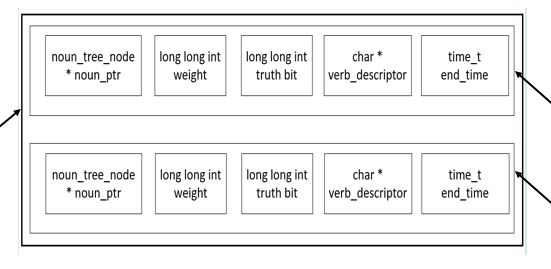
\includegraphics[width=0.5\textwidth]{query_maxheap_nodes.png}}
% \caption{Figure illustrates the Structure of Edge.}
% \label{fig}
% \end{figure}

\section{WORKFLOW}


This section will illustrate how an entry is made in the KG as well as how queries are processed and the graph is traversed.

\begin{figure}[htbp]
\centerline{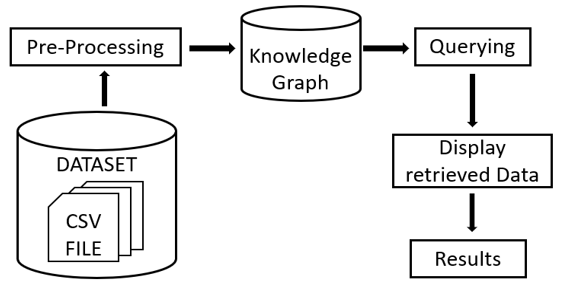
\includegraphics[width=0.5\textwidth , height=4cm]{workflow_5.png}}
\caption{The figure illustrates the workflow}
\label{fig}
\end{figure}
\subsection{\textbf{Example of Entry Creation in the KG}}

Consider the input line: "Computer Science includes a wide range of Data Structures.", which is stored in the CSV file

Pre-processing involves the work of a parser and the insertion of the data points into the KG

Here, the parser will identify "Computer Science" as "noun1" (first noun of the sentence)
and "Data Structures" as "noun2" (second noun of the given input sentence).
Phrases like "includes" will be identified as "verb" and "wide range of" will be classified as "verb-descriptors".

Now there comes a need to store this sentence in the memory where our structural concept
of KG comes into use.
noun1 and noun2 will be inserted into the central AVL noun
tree.

A new noun, $noun3 = noun1 + "\_" + noun2$ gets formed i.e., "Computer Science\_Data Structures"
and will be inserted in the central AVL tree.

Each noun should only be inserted if it does not already exist in the central AVL tree. 
This prevents duplicates, ensuring no redundant nouns are stored, thus optimizing memory usage.

If the noun already exists, connections will be made through the existing noun itself.

The verb "includes" and the verb descriptor "wide range of" are similarly stored in the Verb Tree and Verb descriptor Tree.

Suppose the front weight of the connection is 500 and the back weight is 300.

The memory representation for the given example is as follows: 

\begin{figure}[htbp]
\centerline{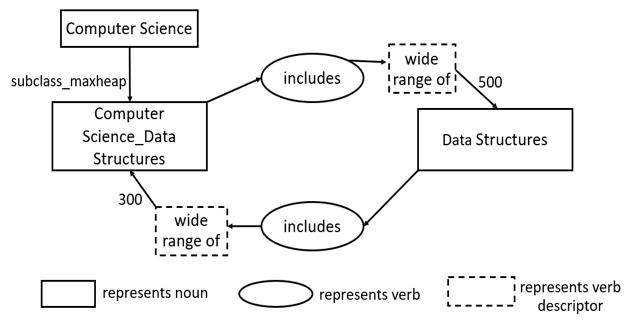
\includegraphics[width=0.52\textwidth , height=6cm]{example_4.png}}
\caption{Figure depicts the memory representation of KG}
\label{fig}
\end{figure}

Further, irrespective of which branch of the central AVL tree the noun gets inserted, 
the connections among them are made, i.e.:

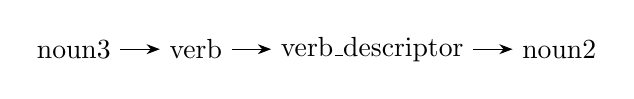
\begin{tikzpicture}[node distance=1.5cm, >=Stealth]
    \node (noun3) {noun3};
    \node (verb) [right=0.5cm of noun3] {verb};
    \node (verb_descriptor) [right=0.5cm of verb] {verb\_descriptor};
    \node (noun2) [right=0.5cm of verb_descriptor] {noun2};

    \draw[->] (noun3) -- (verb);
    \draw[->] (verb) -- (verb_descriptor);
    \draw[->] (verb_descriptor) -- (noun2);
\end{tikzpicture}


In instances where the input line "Computer Science includes a wide range of Data Structures." is 
repeated, instead of creating new connections, the weights associated with the existing connections 
are incremented. This ensures that no redundant data and connections are stored.


\subsection{\textbf{Output Extraction and Querying the KG}}

\subsubsection{Types of Queries in KG}

As an end-user, one may seek the most relevant response to their query. The "Query" stage involves asking the KG various types of queries like :
\begin{itemize}
    \item "Computer Science includes?"
    \item "? includes Data Structures"
    \item "Computer Science includes Data Structures: True or False?"
    \item Or broader queries like: "Describe Computer Science" or "Computer Science?"
\end{itemize}

\subsubsection{Handling Spelling Errors in Queries}
Queries may also contain spelling errors, requiring the system to provide the most relevant output and potentially prompt the user with a "Did you mean?" suggestion.
\\
For example, if a user inputs "Comptr Science includes?", the system should prompt
"Did you mean: Computer Science includes?" 
and proceed based on the user's response.
\\

As developers, it is crucial to handle all these types of queries efficiently. Therefore, functions like search\_noun\_and\_print\_lines() and print\_info\_lines() are used, detailed in subsequent sections.
These are called once the query is processed properly.
\\

\subsubsection{Keeping the Response concise}

Responding to questions like "Describe Computer Science" could overwhelm the user with an extensive amount of data, as the KG may contain thousands of entries related to Computer Science. \\
To manage this, the algorithm prompts the user with a follow-up question: "How many lines of information do you need?" If the user specifies 10 lines, the system will display the 10 most important and weighted connections. 
\\
There is also an option for the system to display all connections in decreasing order of their weights.


Suppose the query analyzer receives the input "Describe Computer Science" and the user also requests: "I want 15 lines of data."
Although the KG may contain thousands of connections, for simplicity, let's assume it has three direct connections as shown in the figure.

\begin{figure}[htbp]
\centering
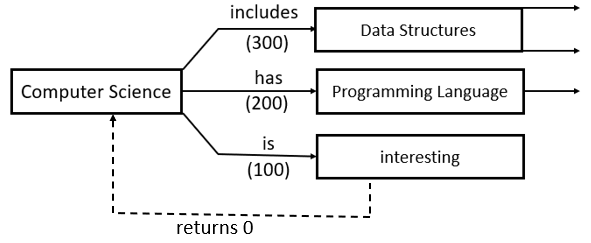
\includegraphics[width=1.0\linewidth,height=5cm]{kg_explanation_example.png}
\caption{Figure illustrates an example of graph traversal}
\label{fig}
\end{figure}

The dotted line "returns 0" is not a connection, and is rather a function call's return value.



The traversal algorithm will prioritize the connections based on their weights. It will allocate lines in proportion to the weights. Here, the proportion is 3 : 2 : 1 (i.e., Data Structures, Programming Language, Interesting).\\ The allocated lines will be distributed to the next nodes in these proportions and this process will continue recursively until all the requested lines have been displayed.\\


Now, in the above example, the total lines allocated are 15. Hence, the following distribution will occur for each connection
\begin{itemize}
\item "Computer Science includes Data Structures": 1 line (for the connection itself), 6 for "Data Structures"
\item "Computer Science has Programming Language": 1 line for itself, 4 for "Programming Language"
\item "Computer Science is Interesting": 1 line for itself, 2 for "Interesting"
\end{itemize}

One line is consumed by the direct connections themselves, and further lines are given for the next-level connections.
Recursive calls of print\_info\_lines() will be made for each of "Data Structures", "Programming Language" and "Interesting".\\

Assuming that "Data Structures" had only 2 direct connections, then 2 lines will get printed (out of the 6 that were allocated to it) and the remaining lines will get re-allocated to "Programming Language".

This means that the recursive call of "Programming Language" will have 8 lines (4 allocated before, 4 reallocated from "Data Structures").

Here "Programming Language" has 1 line to print, hence the remaining 7 lines get re-allocated to "Interesting".

"Interesting" has no lines to print, and hence returns the remaining lines (9 lines) to the noun "Computer Science".

Now, "Computer Science" constructs a traversal queue by utilizing its sub-classes, which are not shown in the figure, and similar recursive calls occur for the subclass nouns.

An important thing to note here is that sub-classes are only traversed for the first level, and further levels do not access subclass heaps. This feature of the algorithm ensures that the same connections are not printed more than once.
In the end, the function returns the number of lines that were printed by it.



\section{Implementation of Querying and Traversal}

The approach for traversing the KG is "Weight Proportional Breadth-First Traversal." Users can interactively query the graph.\\
search\_noun\_and\_print\_lines() takes input: 
\begin{itemize}
\item \textit{input\_noun}: A noun whose connections are to be displayed
\item \textit{total\_lines}: The maximum number of lines to be printed. 
\end{itemize}
print\_info\_lines() also takes similar inputs, but instead of \textit{input\_noun} it takes a pointer to the \textit{input\_noun}


The pseudo-code for both functions are as follows:


\begin{algorithm}
\caption{search\_noun\_and\_print\_lines}
\begin{algorithmic}[1]
\Procedure{\textit{search\_noun\_and\_print\_lines}}{\textit{input\_noun, total\_lines}}
    \State Search for $input\_noun$ in $central\_noun\_tree$
    \State $matching\_noun \gets search\_result\_pointer$
    \If{($matching\_noun$ == NULL)}
        \State Perform another search
        \State Display array of choices to the user
        \For{$selected\_option$ in displayed array}
            \State call print\_info\_lines($selected\_option$)
        \EndFor
    \Else
        \State call print\_info\_lines($matching\_noun$)
    \EndIf
\EndProcedure
\end{algorithmic}
\end{algorithm}


\begin{algorithm}

\caption{print\_info\_lines}
\begin{algorithmic}[1]
\Procedure{\textit{print\_info\_lines}(\textit{total\_lines}, \textit{input\_noun\_ptr})}{}
    \If{(Too few lines allocated for printing)}
        \For{(Most important connections in search\_max\_heap)}
            \State print connection
        \EndFor
        \State return(number of connections printed)
    \Else
        \State construct queue for traversing all connections
        \For{(each $node$ in traversal queue)}
            \State call print\_info\_lines($node$)\
        \EndFor
    \EndIf
    \If{($total\_lines$ not exhausted) and (traversal is in first level)}
        \For{(each $node$ in subclass max\_heap)}
            \State call print\_info\_lines($node$)
        \EndFor
    \EndIf
    \State return(number of lines printed)
\EndProcedure
\end{algorithmic}
\end{algorithm}
\section{ANALYSIS OF ALGORITHMS}
\makeatletter
\renewcommand{\tagform@}[1]{\maketag@@@\textwidth{}\texttt{{...(#1)}}}
\makeatother
\subsection{\textbf{Insertion}}
% Insertion involves parameters that affect the time complexity.
The parameters that affect the time complexity of Insertion are:
\begin{itemize}
    \item Input noun1 string size = $in_{n1}$
    \item Input noun2 string size = $in_{n2}$
\end{itemize}

Firstly, the creation of noun3 is done, which is a concatenation operation, which is a linear time complexity operation
\\
\begin{equation}
T_{\text{concat}}(in_{n1}, in_{n2}) = O(in_{n1} + in_{n2}) = O(n)
\end{equation}

Now, the nouns, verb, and verb descriptor are searched in the trees of the KG:
\begin{itemize}
    \item Number of nouns in the tree = $p$
    \item Length of the string to be searched = $k$
\end{itemize}
In the worst case, searching in the AVL tree will require : 
\begin{equation}
	T_{\text{noun\_searching}}(k, p) = O(k \lg p) = O(n \lg n)
\end{equation}

The time complexity of searching in all the trees(centralized noun AVL tree, database trees that include verb and verb descriptor tree) will also be $O(n \lg n)$:

If the nouns or verbs are not present, then their insertion will cost $O(n \lg n)$ time complexity in the worst case.
\\
Next, we check if the connection already exists. This involves a linear search in various max\_heaps:
\begin{equation}
	T_{\text{searching\_heaps}}(n) = O(n)
\end{equation}
\\
Insertion into various heaps must be done if the edge does not exist.
\begin{equation}
	T_{\text{heap\_insertions}}(n) = O(\lg n)
\end{equation}


\subsection{\textbf{Querying}}

For worst-case analysis, we consider \textit{total\_lines}, the input to these querying functions to be arbitrarily large, and in the context of the C Programming Language, we have considered \textit{total\_lines} to be INT\_MAX.


\subsubsection{\textbf{\texttt{search\_noun\_and\_print\_lines}}}
    Searching for \textit{input\_noun} takes overall $O(k \lg n)$  time where 
    \\k = size of the input string
    \\n = number of nouns (noun nodes) in the noun tree.
    \\If a perfect match isn’t found, the second search will also
take worst case  $O(p \lg n)$ where
    \\p = string in the noun tree that has maximum length
    \\After that, the array of choices is created and displayed. If
the user wants to traverse all the $k$ choices, then the recursive function print\_info\_lines() is called for each choice noun.

\subsubsection{\textbf{\texttt{print\_info\_lines}}}
    \begin{itemize}
        \item \textbf{Too Few lines allocated for printing}: 
\\If $k$ lines are to be printed
and the noun has $m$ connections in its search max heap, ($k \leq m$)
then in the worst case, it will cost:
\begin{equation}
	T(k, m) = O(k\lg m)
\end{equation}

\item \textbf{There are Enough Connections to Traverse}: 
A traversal queue data structure is used for this purpose.
All $k$ connections of the noun are retrieved, and lines are
allocated to them. This operation takes $O(k)$ time. Later,
constructing the queue takes:
\begin{equation}
    T(k) = O(k\lg k) + O(k)
\end{equation}
This is overall $O(k\lg k)$

Once the traversal queue has been constructed, print\_info\_lines() will be called for each node
in the queue.

In the worst case, the starting noun of traversal can be connected with $O(n)$ nodes. Hence, the worst-case time complexity of print\_info\_lines() is
\begin{equation}
    T(n) = O(n\lg n)
\end{equation}
\end{itemize}

search\_noun\_and\_print\_lines() is also worst case $O(n \lg n)$, since its time complexity is asymptotically the same.

Hence, the conclusion is as follows:
\begin{enumerate}
    \item \textbf{Insertion} From equations (1) \ldots 
 \space (4)
    \begin{equation*}
        T_{\text{insertion}}(n) = O(n\lg n) 
    \end{equation*}

    \item \textbf{Querying} From equations (5) \ldots \space (7) 
    \begin{equation*}
        T_{\text{querying}}(n) = O(n\lg n) 
    \end{equation*}
\end{enumerate}


\section{RESULTS}
The graph constructed with the input data consistently produces accurate outputs.\\
The analysis utilized an 11th Gen Intel(R) Core(TM) i5-
1135G7 processor, featuring 8 cores and VT-x virtualization
support.
The insertion algorithm segregates the contexts from the data, supports direct and transitive inference, and can give an accurate KG.

The algorithms presented in section 6 (Algorithm 1 and Algorithm 2) underwent thorough analysis across various parameters, including different numbers of input lines. The analysis focused on the time required to create and query a KG.

Figure 5 put forwards the time analysis of KG, showcasing its remarkably fast response.
\\


\begin{figure}[h!]

\begin{tblr}{colspec={X[c,m]X[c,m]X[c,m]X[c,m]},hlines,column{2}={wd=2.3cm},column{3}={wd=2.1cm}}

Number of input lines & Time taken for KG creation (seconds) & Time taken for querying(seconds) & Total lines displayed\\

\hline
11328&0.3888892&0.008026&6491\\
33984&1.167377&0.013361&11111\\
101952&9.375197&0.021687&27347\\
305856&212.202868&0.059075&82043\\
917568&2795.292009&0.174399&246131
    
\end{tblr}
\end{figure}

% \begin{figure}[htbp]

% \centerline{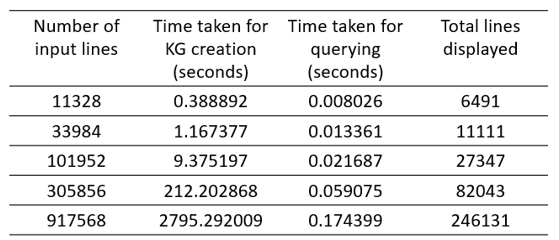
\includegraphics[width=0.5\textwidth , height=4cm]{result_4.png}}
% \caption{Performance analysis of KG}
% \label{fig}
% \end{figure}


% \begin{figure}[htbp]
% \centerline{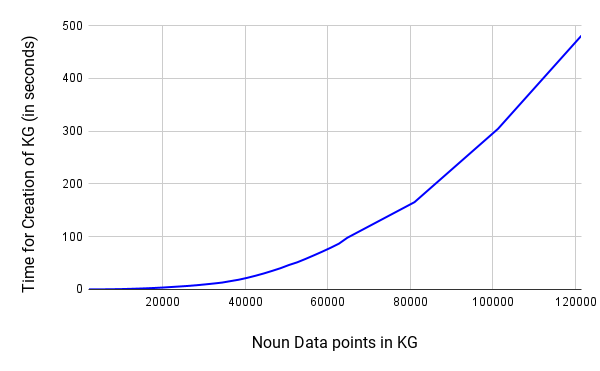
\includegraphics[width=0.5\textwidth , height=6cm]{chart_final.png}}
% \caption{Built Time analysis of the KG}
% \label{fig}
% \end{figure}


\begin{figure}[h!]
    \centering
    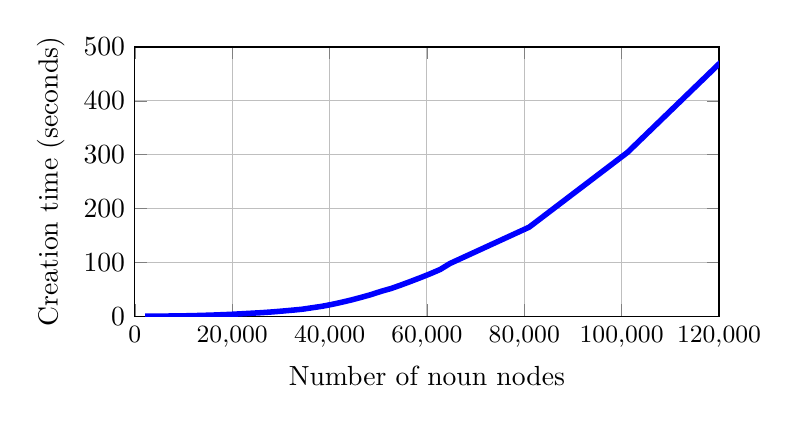
\begin{tikzpicture}
        \begin{axis}[
        %[xlabel style={align=right,text width=3cm},xlabel=A quite long label with a line break]
            xticklabel style={rotate=0,font=\small},
            xlabel={Number of noun nodes},
            ylabel={Creation time (seconds)},
            ytick={0,100,200,300,400,500},
            scaled ticks=false,
            % tick label style={/pgf/number format=fixed}
            xmin=0,
            xmax=120000,
            ymin=0,
            ymax=500,
            grid=major,
            width=9cm,
            height=5cm
        ]
        \addplot[
            color=blue,
            line width=2pt
            ] coordinates {
            (2125,0.042107)
(4145,0.125142)
(6165,0.259413)
(8185,0.458106)
(10205,0.720146)
(12225,1.127179)
(14245,1.622528)
(16265,2.199356)
(18285,2.892098)
(20305,3.706409)
(22325,4.706680)
(24345,5.701934)
(26365,6.757216)
(28385,8.067300)
(30405,9.613722)
(32425,11.237402)
(34445,13.021017)
(36465,15.755038)
(38485,18.452178)
(40505,21.956427)
(42525,25.954854)
(44545,30.323393)
(46565,35.174854)
(48585,40.285606)
(50605,46.270065)
(52625,51.414076)
(54645,57.849135)
(56665,64.645857)
(58685,71.634150)
(60705,78.942484)
(62725,86.782613)
(64745,97.932170)
(81005,165.387548)
(101205,304.285815)
(121405,480.884535)

        };
        \end{axis}
    \end{tikzpicture}
    \caption{Graph explains the performance analysis of creating the graph}
    \label{fig:simple_graph}
\end{figure}

As depicted in figure 6, the graph conforms to the mathematical analysis of the algorithm presented in this paper.

\section{CONCLUSION}
This study puts forward a fundamental kernel-level implementation of a KG. 
The proposed system demonstrates that querying a KG, which stores millions of data points, is remarkably fast. 
The structure of the KG is designed to ensure that accurate relationships are provided for given queries, achieving 100\% accuracy.
\\
The present work can be improved by integrating KG with NLP, which would enable the construction of KG from unstructured data.

% \section{ACKNOWLEDGEMENTS}
% The authors would like to express their sincere gratitude to Dr. Pratiksha Deshmukh, Professor, Department of CSE, COEP Technological University for her invaluable assistance and guidance throughout the course of this research project.


\begin{thebibliography}{00}

\bibitem{b1} Samadrita Ghosh, "Knowledge Graphs — What, Why, and How", 2022, available at: \url{https://samadritaghosh.medium.com/knowledge-graphs-what-why-and-how-84f920316ca5}
\bibitem{b2} Da Xu, Chuanwei Ruan et al, "Product Knowledge Graph Embedding for E-commerce"  January 2020 available at: \url{https://doi.org/10.1145/3336191.3371778}

\bibitem{b3} Arun Krishnan "Making search easier", Amazon Blog, August 17, 2018, available at: \url{https://blog.aboutamazon.com/innovation/making-search-easie}

\bibitem{b4} R. J. Pittman, Amit Srivastava et al, "Cracking the Code on Conversational Commerce", eBay Blog,  April 6, 2017, available at:  \url{https://www.ebayinc.com/stories/news/cracking-the-code-on-conversational-commerce/}

\bibitem{b5}Qi He, Bee-Chung Chen, and Deepak Agarwal "Building The
LinkedIn Knowledge Graph", LinkedIn Blog,  October 6, 2016, available at: \url{https://engineering.linkedin.com/blog/2016/10/building-the-linkedin-knowledge-graph}


\bibitem{b7} Ergeta Muca, "Introduction to Knowledge Graphs and their Applications" Published in
Analytics Vidhya Dec 10, 2019, available 
at : \url{https://medium.com/analytics-vidhya/introduction-to-knowledge-graphs-and-their-applications-fb5b12da2a8b}

\bibitem{b8} Aidan Hogan, Eva Blomqvist, et al, "Knowledge Graphs", ACM
Computing Surveys, 11 September 2021,  available at: \url{https://arxiv.org/pdf/2003.02320}

\bibitem{b9} Brian Kernighan, Dennis Ritchie "The C Programming Language", 2nd edition, 8 April 1988

\bibitem{b10} Samadrita Ghosh, "Knowledge Graphs — What, Why, and How", medium, Dec 19, 2022, available at: \url{https://samadritaghosh.medium.com/knowledge-graphs-what-why-and-how-84f920316ca5}

\bibitem{b11} Fabricated Data Set available at : \url{https://github.com/Arnav2Prasad/C_Knowledge_Graph_project}

\bibitem{b12} Foundations of Modern Query Languages for Graph Databases, available at: \url{https://dl.acm.org/doi/pdf/10.1145/3104031}

\bibitem{b16} Helena Cousijn, Ricarda Braukmann et al. Connected Research: The Potential of the PID Graph, Patterns, Volume 2, Issue 1, 2021, 100180, ISSN 2666-3899, available at: \url{https://www.sciencedirect.com/science/article/pii/S2666389920302440}

\bibitem{b17}Liu, Yu, and Hua "Context-Aware Temporal Knowledge Graph Embedding", October 2019
available at: \url{https://www.researchgate.net/publication/337245161_Context-Aware_Temporal_Knowledge_Graph_Embedding}

\bibitem{b18}Rana Hussein, Dingqi Yang, and Philippe Cudré-Mauroux, 2018. Are Meta-Paths Necessary? available at: \url{https://dl.acm.org/doi/10.1145/3269206.3271777}



\end{thebibliography}
\end{document}  
